\documentclass[compress]{beamer}
\usetheme{Warsaw}
\usecolortheme{seagull}
\setbeamertemplate{headline}{}
\beamertemplatenavigationsymbolsempty
\useoutertheme{infolines}

\usepackage{lipsum}
\setbeamersize{text margin left=10pt,text margin right=10pt}
\setbeamertemplate{enumerate items}[default]
\setbeamertemplate{itemize items}[default]

%\addtobeamertemplate{navigation symbols}{}{%
%    \usebeamerfont{footline}%
%    \usebeamercolor[fg]{footline}%
%    \hspace{1em}%
%    \insertframenumber/\inserttotalframenumber
%}

\usepackage{graphicx}
\graphicspath{{/Users/jlochman/Desktop/Diploma-thesis/Chapter3/}}
\usepackage{epstopdf}
\usepackage{booktabs} 
\usepackage{courier}

\PassOptionsToPackage{demo}{graphicx}
\def\Put(#1,#2)#3{\leavevmode\makebox(0,0){\put(#1,#2){#3}}}

\newcommand{\GeV}{\,\text{GeV}}
\newcommand{\TeV}{\,\text{TeV}}
\newcommand{\pt}{p_{T}}

\title[High $\pt$ jets]{Hight $\pt$ jets in Run II of the ATLAS Experiment} 
\author{Jan Lochman}
\institute[FNSPE CTU] 
{
Czech Technical University \\ 
\medskip
\textit{jan.lochman@cern.ch} \\
\medskip
\medskip
ATLAS Meeting \\ 
\medskip
}
\date{\today}

\begin{document}

\section{Introduction}

%------------------------------------------------

\begin{frame}
\titlepage 
\end{frame}

%------------------------------------------------

\begin{frame}
\frametitle{My Analysis} 
\begin{itemize}
  \item Inclusive jet double differential cross section in $\pt$ and rapidity
    $y$ (inclusive means $pp \rightarrow$ jet + anything) in Run~II of the ATLAS
    Experiment (meaning $\sqrt{s}=13\TeV$)
  \item Data 
    \begin{enumerate}
      \item Monte Carlo  generated events of $pp$ collisions at
        $\sqrt{s}=13\TeV$. 
      \begin{itemize}
        \item Collisions generated with \textsc{Pythia8} (particle level)
        \item ATLAS Detector response obtained with \textsc{Geant4} full
          simulation (detector level)
      \end{itemize}
      \item NLO QCD predictions (parton level)
    \end{enumerate}
  \item Cross section corrected from the detector to the particle level in two
    steps
    \begin{itemize}
      \item Calibration
      \item Unfolding
    \end{itemize}
  \item Particle level cross section from \textsc{Pythia8} (LO QCD) compared
    with the parton level NLO QCD cross section prediction.
\end{itemize}
\end{frame}

\section{Jets}
\subsection{Introduction}

\begin{frame}
\frametitle{Jet Necessity}
\begin{itemize}
  \item Gluon radiation cross section
\begin{equation*}
  \sigma_{q \rightarrow qg} \sim \frac{d\theta}{|\sin\theta|}
  \frac{dE_k}{E_k}
\end{equation*}
  \item Divergences
    \begin{itemize}
      \item Infrared ($E_k = 0$)
      \item Collinear ($\theta = 0$)
    \end{itemize}
  \item Good observables are IR and collinear safe, i.e. they are not
    affected by soft and collinear splittings of final state partons.
\end{itemize}
\begin{figure}[b]
  \centering
  
\includegraphics[width=0.8\textwidth]{{../PrezentationATLASmeeting/gluonRadiation}.png}
\end{figure}
\end{frame}

\subsection{Jet Algorithms}

\begin{frame}
\frametitle{Jet Requirements}
  \begin{itemize}
    \item Jet can be naively seen as a group of collimated particles
    \item Jet algorithm: A prescription, how particles (or other objects) are clustered
          into separate jets. It should fulfill
  \end{itemize}
\begin{columns}[onlytextwidth]
  \begin{column}{0.6\textwidth}
      \begin{itemize}
        \item Infrared safety  
          
          The presence of an additional soft particle
          should not affect the recombination of particles into a jet.
        \item Collinear safety  
          
          Jet reconstruction should not depend on the
          fact, if the energy is carried by one particle, of if the particle is
          split into more collinear particles.
      \end{itemize}
  \end{column}
  \begin{column}{0.4\textwidth}
    \begin{figure}[b]
      \centering
      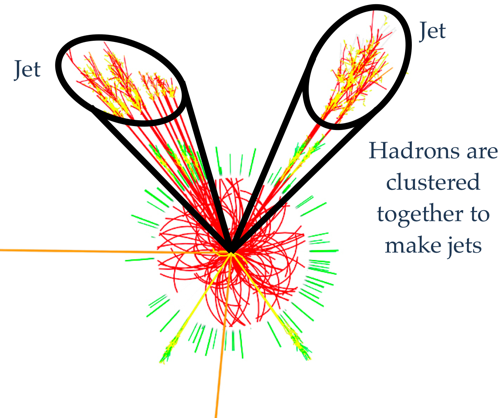
\includegraphics[width=0.9\textwidth]{{../PrezentationATLASmeeting/clustering}.png}
    \end{figure}
  \end{column}
\end{columns}
\end{frame}

\begin{frame}
\frametitle{Fixed Cone Jet Algorithms}
\begin{itemize}
  \item The most illustrative jet algorithms. Different modifications.
  \item Used in Tevatron. Not used in ATLAS. 
\end{itemize}
\begin{columns}[onlytextwidth]
  \begin{column}{0.4\textwidth}
    \begin{figure}[t]
      \centering
      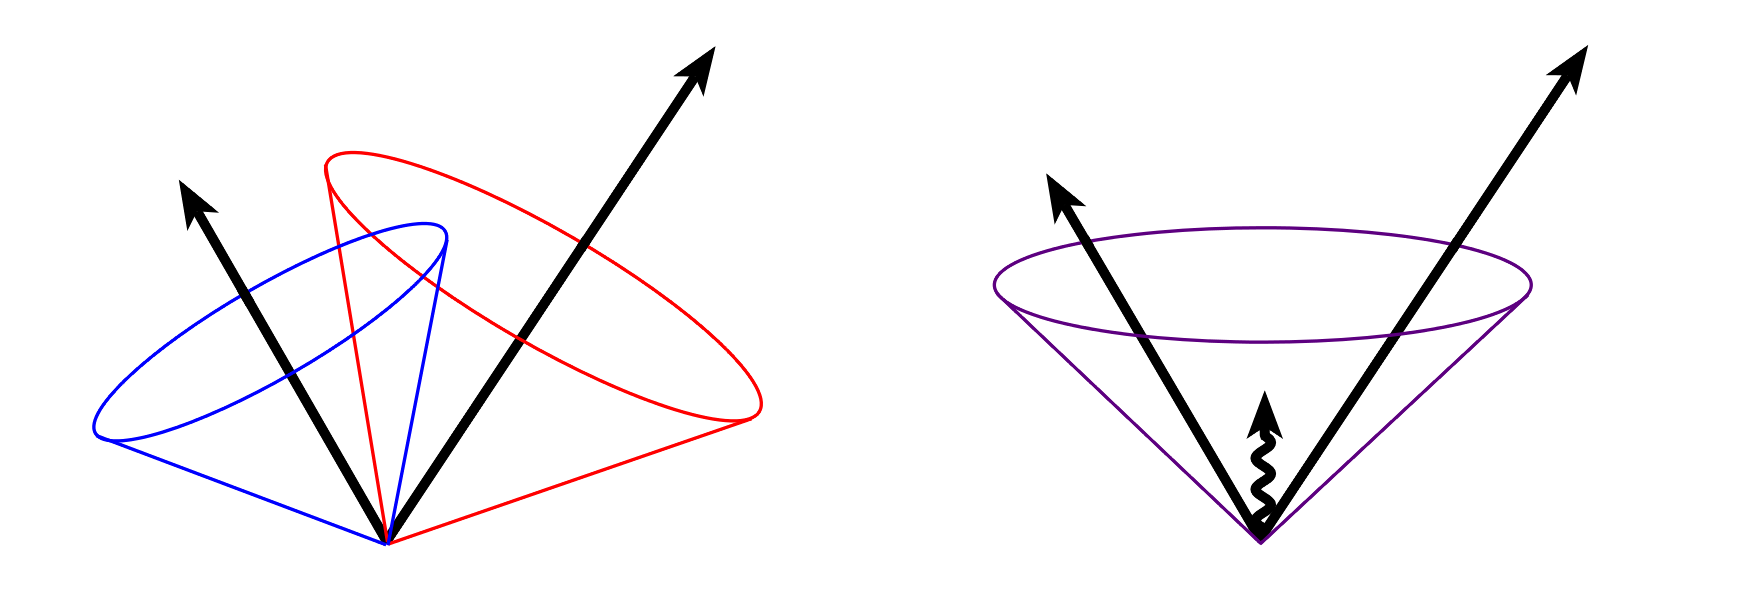
\includegraphics[width=0.9\textwidth]{{../Chapter2/IRsafety}.png}
      \\
      infrared unsafety
      \\
      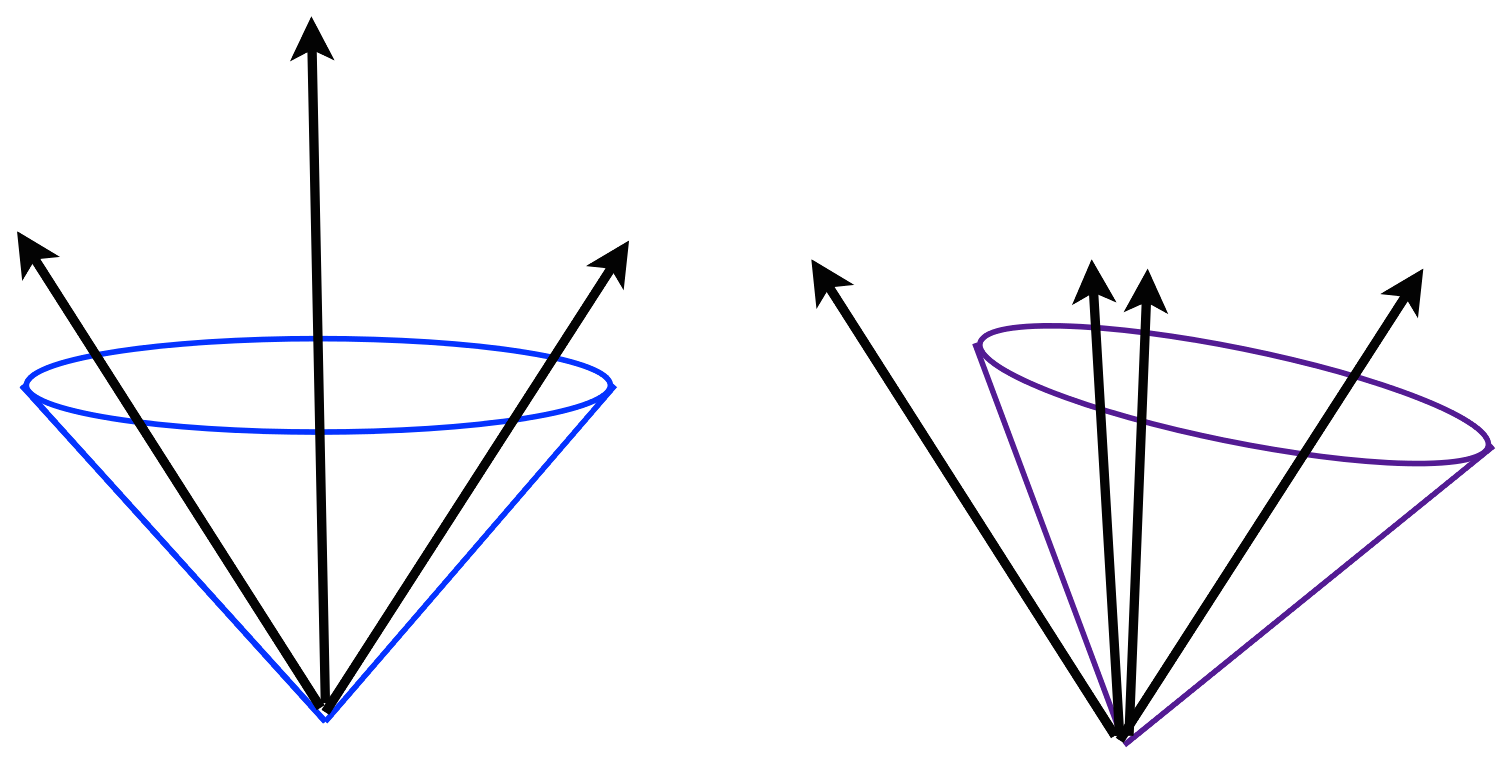
\includegraphics[width=0.9\textwidth]{{../Chapter2/ColSafety}.png}
      \\
      collinear unsafety
    \end{figure}
  \end{column}
  \begin{column}{0.6\textwidth}
    \begin{enumerate}
      \item Take particle with highest $\pt > \pt^{cutoff}$
      \item Recombine all particle within the fixed cone 
      \item Update cone direction
      \item If direction have changed go to 2, else you have a jet
      \item Go to 1 until there is no particle left with $\pt > \pt^{cutoff}$
    \end{enumerate}
  \end{column}
\end{columns}
\end{frame}

\begin{frame}
\frametitle{Anti-$k_t$ Jet Algorithm}
\begin{enumerate}
  \item For each input object $i$ and all pairs of input objects $(i,j)$
    calculate
    \begin{equation*}
      d_i = p_{T,i}^{-2} \quad , \quad
      d_{ij} = \min \left( p_{T,i}^{-2}, p_{T,j}^{-2} \right)
      \frac{ \Delta y^2 + \Delta \phi^2 }{R^2} \quad \quad
      (R=0.4)
    \end{equation*}
  \item Find minimum $d_{min}$ between all $d_{ij}$ and $d_i$
  \begin{itemize}
    \item $d_{min}$ is between $d_{ij}$'s.
      
      Recombine $i$, $j$ into a new object $k$. Remove $i$, $j$ from the list,
      add $k$ to the list.

    \item $d_{min}$ is between $d_i$'s.
      
      Object $i$ is a jet. Remove $i$ from the list.
  \end{itemize}
  \item Go to 1 until all input objects are part of a jet.
\end{enumerate}
This jet algorithm is both infrared and collinear safe
\end{frame}

\begin{frame}
\frametitle{Anti-$k_t$ Jet Algorithm}
\begin{figure}[t]
  \centering
  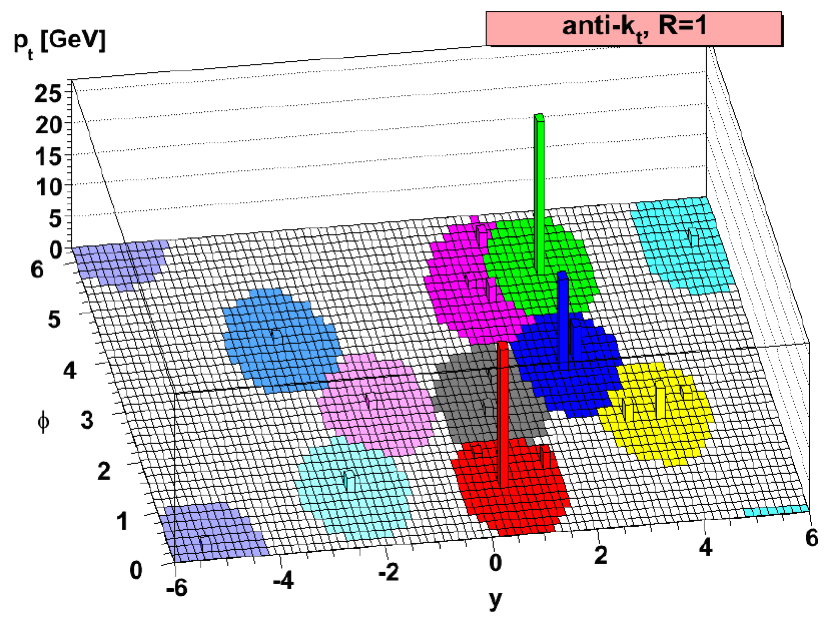
\includegraphics[width=0.8\textwidth]{{../Chapter2/JetRecombination2}.png}
\end{figure}
\end{frame}

\section{Jet Reconstruction}
\subsection{Parton, Particle and Detector Levels}

\begin{frame}
\frametitle{Jet Reconstruction}
Jet can be defined on three different levels of collisions
\begin{itemize}
  \item Parton level - quarks, gluons and other particles created just after the
    collision. Directly connected to the QCD processes
  \item Particle level - particles created by the hadronization. 
  \item Detector level - from recorded signal. Detector imperfections cause a
    distortion of observables.
\end{itemize}
\begin{figure}[b]
  \centering
  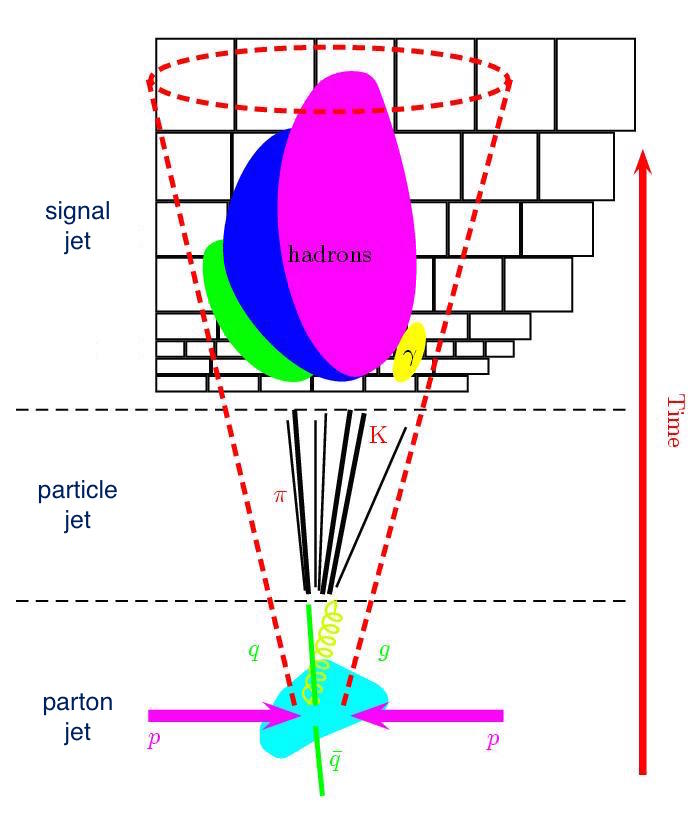
\includegraphics[width=0.7\textwidth]{{../Chapter2/JetPhases}.png}
\end{figure}
\end{frame}

\subsection{Jet Corrections}

\begin{frame}
\frametitle{Jet Corrections}
\begin{itemize}
  \item Correct observables derived from detector level to particle level by
    removing the detector effects
  \item Two main procedures - Calibration and Unfolding
  \item Both procedures are trained on Monte Carlo data
\end{itemize}
\begin{figure}[b]
  \centering
  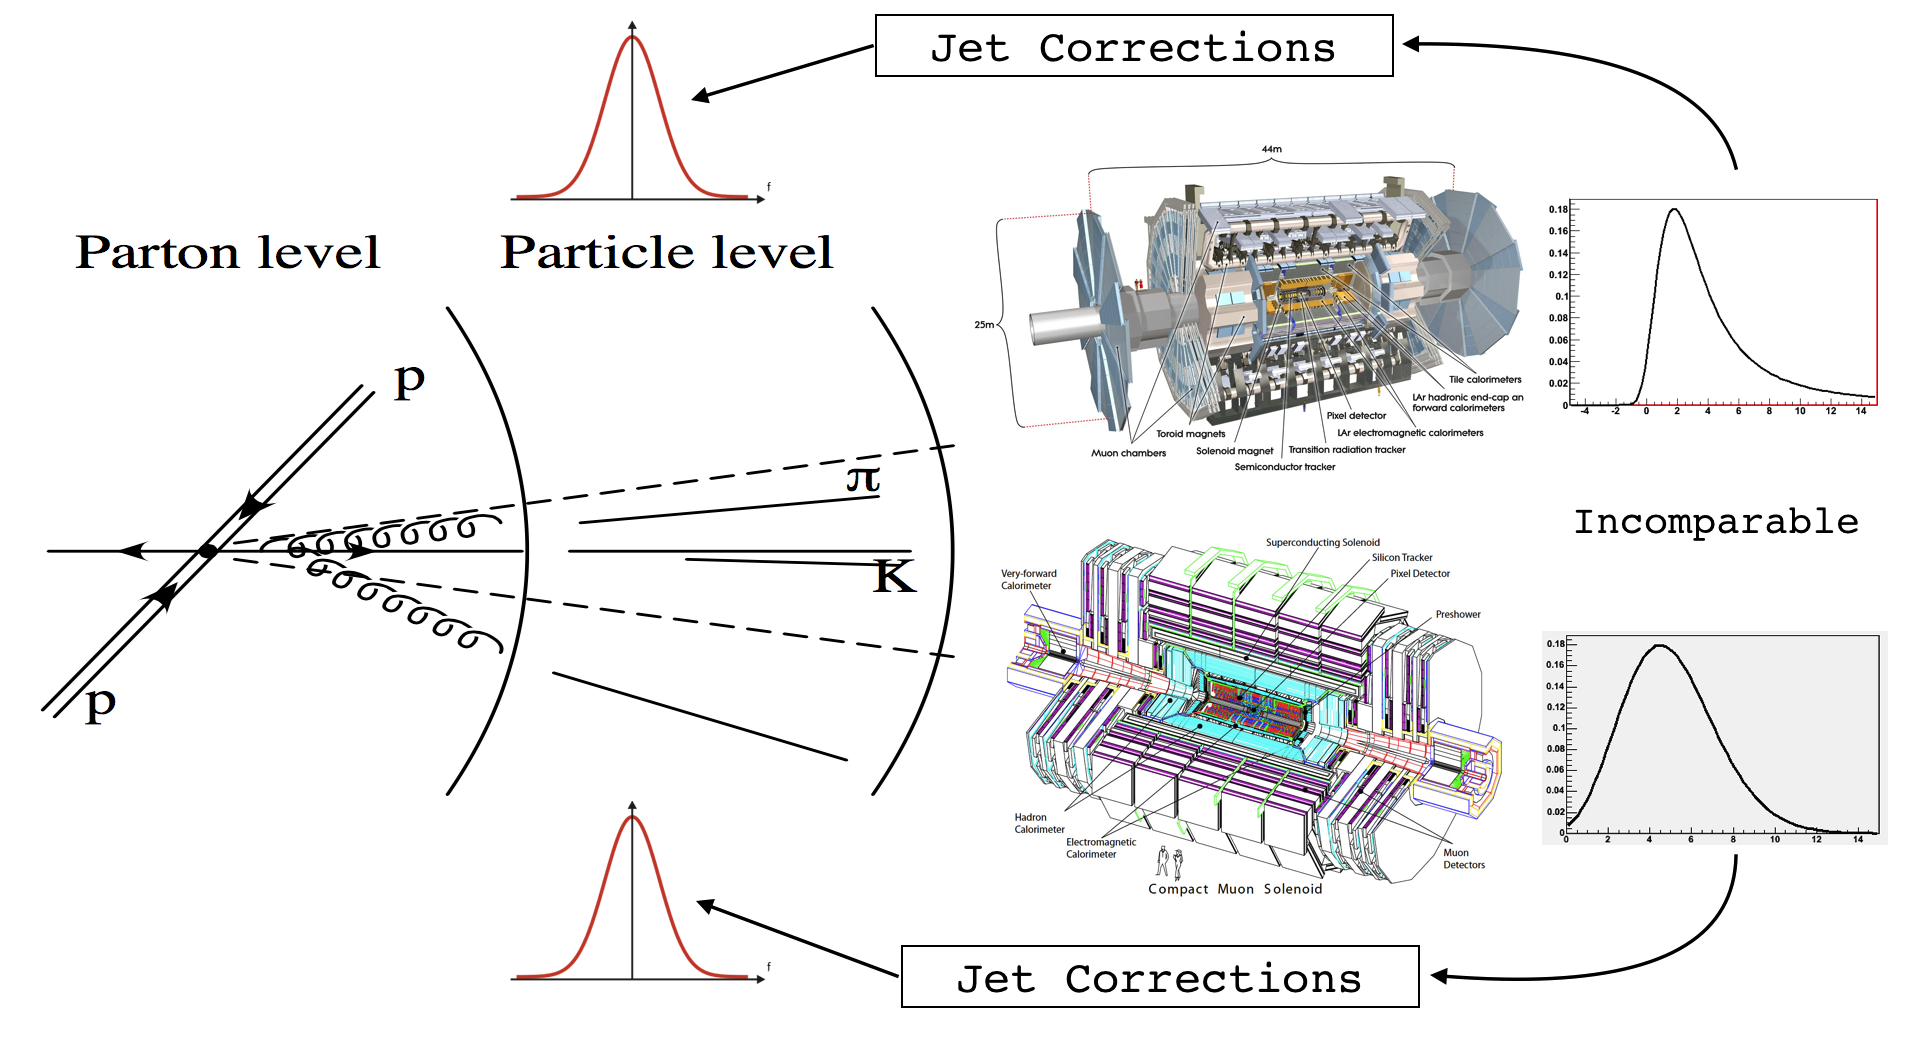
\includegraphics[width=0.85\textwidth]{{../PrezentationATLASmeeting/JetCorrections}.png}
\end{figure}
\end{frame}

\subsection{Calibration}

\begin{frame}
\frametitle{Calibration}
\begin{itemize}
  \item Modifies the kinematic properties of individual jets - the most important
    correction: Energy
  \item Tries to minimize the calorimeter non-compensation, noise, losses in dead
    material and cracks, longitudinal leakage and particle deflection in magnetic
    field.
  \item Universal for each jet analysis. Uses the standard
    \textsc{ApplyJetCalibration} library.
\end{itemize}
\begin{figure}[b]
  \centering
  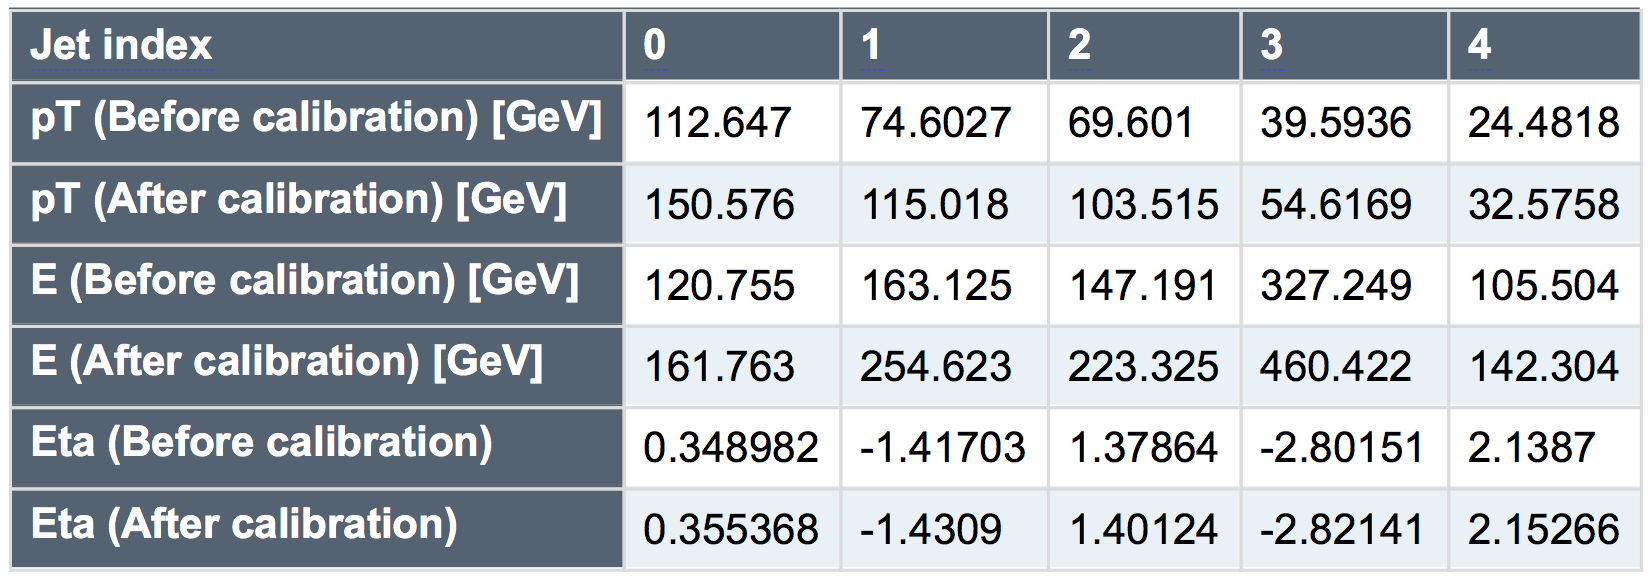
\includegraphics[width=0.9\textwidth]{{../PrezentationATLASmeeting/JetCalibration}.png}
\end{figure}
\end{frame}

\subsection{Unfolding}

\begin{frame}
\frametitle{Unfolding}
\begin{itemize}
  \item Corrects the observables from detector level, to observables on particle
    level. 
  \item Tries to minimize the effects of detector finite resolution.
  \item Analysis dependent.
\end{itemize}
\begin{figure}[b]
  \centering
  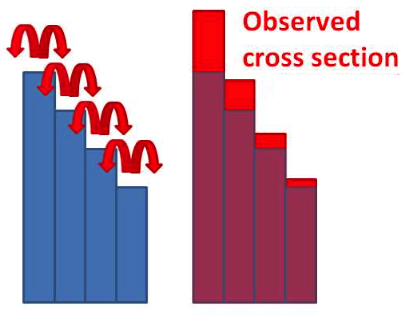
\includegraphics[width=0.39\textwidth]{{../PrezentationATLASmeeting/UnfoldingEffect}.png}
  \includegraphics[width=0.6\textwidth]{{SignalVSTruth}.eps}
\end{figure}
\end{frame}

\begin{frame}
\frametitle{Unfolding - Mathematical Formulation}
\begin{itemize}
  \item I want: $f(\pt)$ (distribution of inclusive jet $\pt$ for $\pt \in
    \langle a, b \rangle$)
  \item From detector level I get: $g(x)$ (distribution of unphysical variable
    $x$)
  \begin{equation*}
    g(x) = \int_a^b A(x,\pt) f(\pt) d\pt
  \end{equation*}
  \item Detector smearing described by $A(x,\pt)$
  \item Luckily $g(x)$ and $f(\pt)$ are for practical purpose discretized and in
    analysis, I assume $x \in \langle a, b \rangle$, $N(i) \subset \langle
    a , b \rangle$ 
  \begin{equation*}
    g_i = \int_{N(i)}g(x)dx \quad , \quad f_i = \int_{N(i)}f(\pt)d\pt
  \end{equation*}
  \item So the response of the detector is described by a simple matrix equation
    \begin{equation*}
      g = A f
    \end{equation*}
  \item Here $A$ is called the Transfer Matrix
\end{itemize}
\end{frame}

\section{Data Analysis}
\subsection{Data Characteristics}

\begin{frame}
\frametitle{Data Characteristics}
\begin{itemize}
  \item $pp$ collisions at $\sqrt{s}=13\TeV$, anti-$k_t$ jet algorithm with
    $R=0.4$, CT10 PDFs, AU2
  \item Measuring of inclusive jet double differential cross section in $\pt$
    and rapidity $y$ \end{itemize}
\begin{columns}[onlytextwidth]
  \begin{column}{0.5\textwidth}
\begin{itemize}
  \item Parton level - cross section prediction calculated with NLOJET++ program
    (NLO~QCD)
  \item Particle level - events generated by \textsc{Pythia8} (LO~QCD)
  \item Detector level - detector response on \textsc{Pythia8} events obtained
    by \textsc{Geant4} full detector simulation. 
\end{itemize}
  \end{column}
  \begin{column}{0.5\textwidth}
\begin{figure}[b]
  \centering
  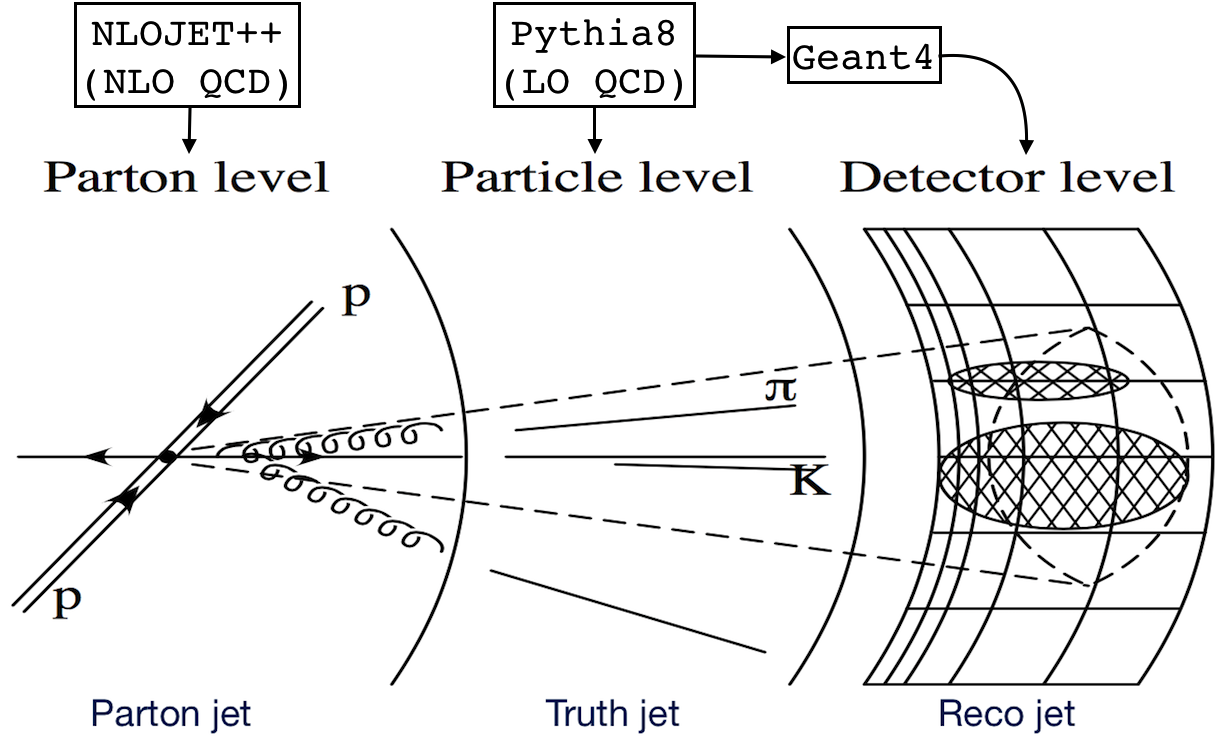
\includegraphics[width=\textwidth]{{../PrezentationATLASmeeting/DataChar}.png}
\end{figure}
  \end{column}
\end{columns}
\end{frame}

\begin{frame}
\frametitle{\textsc{Pythia8} Data Characteristics}
\begin{itemize}
  \item Events were generated in a slices according to the leading truth
      jet $\pt$.
  \item Slices differ in event weight which is for all event calculated as
  \begin{equation*}
    \text{weight} = \frac{\text{(Cross-section)} \cdot \text{(Filter
      Efficiency)} \cdot w_0}{\text{(\# events)}} 
    \end{equation*}
  \item $w_0$ is additional weight factor stored in \texttt{EventInfoAux}
    container
\end{itemize}
  \small
  \begin{table}
  \centering
  \begin{tabular}{|c|rcr|c|c|c|}
    \hline 
     JZ & \multicolumn{3}{|c|}{$\pt$ range (GeV)} & Cross-section (fb) & Filter Efficiency & \# events  \\ 
    \hline
    \hline
		 JZ0W &     0 & - &    20 & 7.8420e+13 & 9.7193e-01 & 3498000 \\ 
    \hline
		 JZ1W &    20 & - &    80 & 7.8420e+13 & 2.7903e-04 & 2998000 \\
    \hline
		 JZ2W &    80 & - &   200 & 5.7312e+10 & 5.2261e-03 & 500000  \\
    \hline
		 JZ3W &   200 & - &   500 & 1.4478e+09 & 1.8068e-03 & 499500  \\
    \hline
		 JZ4W &   500 & - &  1000 & 2.3093e+07 & 1.3276e-03 & 477000  \\
    \hline
		 JZ5W &  1000 & - &  1500 & 2.3793e+05 & 5.0449e-03 & 499000  \\
    \hline
		 JZ6W &  1500 & - &  2000 & 5.4279e+03 & 1.3886e-02 & 493500  \\
    \hline
		 JZ7W &  2000 & + &       & 9.4172e+02 & 6.7141e-02 & 497000  \\
    \hline 
  \end{tabular}
\end{table}
\normalsize
\end{frame}

\subsection{Event Selection}

\begin{frame}
\frametitle{Event Selection}
\begin{itemize}
  \item \textbf{$\mathbf{\pt}$ Cut}
  
    Reco and truth jets with $\pt > 15 \GeV$ were kept.
  \item \textbf{$\mathbf{y}$ Cut}

    Reco and truth jets with $|y| < 4$ were kept.

  \item \textbf{Zero Jet (0-jet) Cut}
    
    Events with at least one reco and one truth jet, after the
    $\pt$ and $y$ cuts, are considered.
    
  \item \textbf{Leading Ratio (LR) Cut}

    If $0.6 < LR < 1.4$ the event is considered
    \begin{equation*}
      LR = p_{T,leading}^{reco} / p_{T,leading}^{truth} 
    \end{equation*}
\end{itemize}
\end{frame}

\begin{frame}
\frametitle{Event Selection - Truth Jets}
\begin{figure}[b]
  \centering
  \includegraphics[width=\textwidth]{{TruthCutting}.eps}
\end{figure}
\end{frame}

\begin{frame}
\frametitle{Event Selection - Reco Jets}
\begin{figure}[b]
  \centering
  \includegraphics[width=\textwidth]{{SignalCutting}.eps}
\end{figure}
\end{frame}

\subsection{Jet Matching}

\begin{frame}
\frametitle{Jet Matching}
\begin{itemize}
  \item In each event, for each truth jet, the corresponding reco jet has to be found.
  \item I have used angular matching
    \begin{itemize}
      \item For each pair $(i,j)$ of reco and truth jets
        \begin{equation*}
          dR_{ij} = \sqrt{d\phi_{ij}^2 + dy_{ij}^2}
        \end{equation*}
      \item If $\min(dR_{ij}) = dR_{pq} < dR^{cutoff} = 0.2$ the jets (p,q) were
        matched and further not assumed
      \item Matching was done, when $\min(dR_{ij}) < dR^{cutoff}$ was not
        satisfied or all of the reco or truth jets were matched.
    \end{itemize}
\end{itemize}
\end{frame}

\begin{frame}
\frametitle{Jet Matching - Truth Jets}
\begin{figure}[b]
  \centering
  \includegraphics[width=\textwidth]{{TruthMatching}.eps}
\end{figure}
\end{frame}

\begin{frame}
\frametitle{Jet Matching - Reco Jets}
\begin{figure}[b]
  \centering
  \includegraphics[width=\textwidth]{{SignalMatching}.eps}
\end{figure}
\end{frame}

\subsection{Unfolding}

\begin{frame}
\frametitle{Inputs for Unfolding}
Unfolding (calibrated reco spectrum) $\approx$ truth spectrum
\begin{itemize}
  \item Inputs for unfolding procedure are
    \begin{itemize}
      \item Matching efficiencies - describing the ratio of matched jets to all jets
      \item Transfer matrix $A_{ij}$ - containing the number of reco jets in bin $i$ with
        a matched truth jets generated in bin $j$
    \end{itemize}
  \item To deal with the double binning (in $\pt$ and $y$), I use two approaches
    to the unfolding
\end{itemize}
\begin{enumerate}
  \item Simple unfolding

    Matching jets within different rapidity bins is not allowed. There are 8
    independent 46x46 transfer matrices, one for each rapidity bin (46 = number
    of $\pt$ bins)
  \item 2D unfolding

    Matching within different rapidity bins allowed. Only one 368x368 transfer
    matrix ($368=8 \times 48$)
\end{enumerate}
\end{frame}

\begin{frame}
\frametitle{Transfer Matrices}
\begin{columns}[onlytextwidth]
  \begin{column}{0.5\textwidth}
    \begin{figure}[H]
      \centering
    2D unfolding
      \includegraphics[width=\textwidth]{{unfold_matrix_all}.eps}
    \end{figure}
  \end{column}
  \begin{column}{0.5\textwidth}
    \begin{figure}[H]
      \centering
    Simple unfolding
      \includegraphics[width=\textwidth]{{unfold_matrix_firstBin}.eps}
    \end{figure}
  \end{column}
\end{columns}
\end{frame}

\begin{frame}
\frametitle{Slices in Transfer Matrix of 2D Unfolding}
\Put(265,20){\color{blue}\includegraphics[height=3cm]{{unfold_matrix_all}.eps}}
\begin{figure}[b]
  \raggedright
  \includegraphics[width=0.8\textwidth]{{UnfoldMatrixSlices11}.eps}
\end{figure}
\end{frame}

\begin{frame}
\frametitle{Matching Efficiencies}
\begin{columns}[onlytextwidth]
  \begin{column}{0.5\textwidth}
    \begin{figure}[H]
      \centering
    Truth jets
      \includegraphics[width=\textwidth]{{MatchEffSimpe2DSignal0Compare}.eps}
    \end{figure}
  \end{column}
  \begin{column}{0.5\textwidth}
    \begin{figure}[H]
      \centering
    Reco jets
      \includegraphics[width=\textwidth]{{MatchEffSimpe2DTruth0Compare}.eps}
    \end{figure}
  \end{column}
\end{columns}
\end{frame}

\begin{frame}
\frametitle{Steps of Unfolding}
Unfolding procedure can be divided into three main steps
\begin{enumerate}
  \item Input data are multiplied by the matching efficiencies of reco jets
  \item Transfer matrix is used to correct data spectrum for detector effects. I
    use the Iterative Dynamical Stabilized unfolding method with one iteration
  \item The spectrum obtained by the step 2 is divided by the matching
    efficiencies of truth jets, in order to correct resulting spectrum for the
    unmatched truth jets
\end{enumerate}
\end{frame}

\begin{frame}
\frametitle{Unfolding Results}
\begin{columns}[onlytextwidth]
  \begin{column}{0.5\textwidth}
    \begin{figure}[H]
      \centering
    Reco and Unfolded vs. Truth Spectrum
      \includegraphics[width=\textwidth]{{SignalUnfolded_VS_Truth0Compare}.eps}
    \end{figure}
  \end{column}
  \begin{column}{0.5\textwidth}
    \begin{figure}[H]
      \centering
    Simple and 2D unfolded vs. Truth Spectrum
      \includegraphics[width=\textwidth]{{UnfoldedSimpleComplex_VS_Truth0Compare}.eps}
    \end{figure}
  \end{column}
\end{columns}
\end{frame}

\section{NLO QCD Predictions}
\subsection{Introduction}

\begin{frame}
\frametitle{NLO QCD Prediction}
\begin{itemize}
  \item NLO QCD predictions on parton level for $\sqrt{s}=8\TeV$ and
    $\sqrt{s}=13\TeV$
  \item Theoretical uncertainties which are taken into account
  \begin{itemize}
    \item \textbf{Scale uncertainty}

      Choice of renormalization and factorization scales, including
      neglecting the higher order terms beyond the NLO
    \item \textbf{$\alpha_S$ uncertainty}

      Because of experimental measurements of $\alpha_S$.
    \item \textbf{PDF uncertainty}

      Prediction depends on the concrete choice of a PDF
  \end{itemize}
  \item Other uncertainties (not so significant)
  \begin{itemize}
    \item \textbf{Nonperturbative corrections uncertainty}

      Hadronization and Underlying Event corrections.
    \item \textbf{Electroweak corrections uncertainty}

      Next to the QCD processes, the electroweak processes should be assumed.
  \end{itemize}
\end{itemize}
\end{frame}

\subsection{Prediction Properties}

\begin{frame}
\frametitle{NLO Systematic Errors}
\begin{columns}[onlytextwidth]
  \begin{column}{0.5\textwidth}
    \begin{figure}[H]
      \centering
      $\sqrt{s}=8\TeV$
      \includegraphics[width=\textwidth]{{NLO_Systematics8_TeV0}.eps}
    \end{figure}
  \end{column}
  \begin{column}{0.5\textwidth}
    \begin{figure}[H]
      \centering
      $\sqrt{s}=13\TeV$
      \includegraphics[width=\textwidth]{{NLO_Systematics13_TeV0}.eps}
    \end{figure}
  \end{column}
\end{columns}
\end{frame}

\begin{frame}
\frametitle{Comparison of NLO QCD Predictions}
\begin{figure}[b]
  \centering
  \includegraphics[width=\textwidth]{{PredictionCompare0}.eps}
\end{figure}
\end{frame}

\subsection{Comparison with \textsc{Pythia8}}

\begin{frame}
\frametitle{Comparison of LO and NLO QCD}
\begin{figure}[b]
  \centering
  \includegraphics[width=0.8\textwidth]{{Truth_VS_Prediction0Compare}.eps}
\end{figure}
\end{frame}

\section{Conclusion}

\begin{frame}
\frametitle{Inclusive Jet Conclusions}
\begin{block}{Why Inclusive Jets?}
  They Cover wide range of momentum transfers ($\sim 1 \GeV - 1 \TeV$ on
  the LHC) $\rightarrow$ predictions sensitive to
  the properties of the running coupling constant $\alpha_S$

  They probe the structure of proton at small distance scales 
  \begin{equation*}
    \lambda \sim 1/\pt \sim \TeV^{-1} \sim 10^{-19}\,\text{m}
  \end{equation*}

  They contribute to our understanding of PDF

  They appreciate the increase in the transverse momentum as no other physics
  process observed on hadron colliders
\end{block}
\end{frame}

\begin{frame}
\frametitle{Thesis Conclusions}
\begin{block}{Unfolding}
  Two approaches were probed.
  
  No significant differences between these two approaches imply, for the real
  analysis, the Simple Unfolding approach should be used for its simpler
  implementation.

  Agreement of the unfolded $\pt$ spectra with the truth $\pt$ spectra up to
  systematic error $<10^{-3}\,\%$.
\end{block}
\begin{block}{LO and NLO QCD}
  Significant differences showing the influence of the NLO QCD processes on
  physical observables.
\end{block}
\end{frame}

\end{document} 
